\chapter{Rodzaje aplikacji internetowych}
\label{roz2}
%=================================================================================================
\section{Aplikacje internetowe}
Szybko rosnąca popularność internetu~w latach 90. XX wieku sprawiła, że poza prostymi stronami \textit{HTML}\footnote{HTML(ang. \textit{HyperText Markup Language}), hipertekstowy język znaczników powszechnie używany do tworzenia stron internetowych. Źródło \url{https://www.w3.org/TR/html4/}} zaczęto budować bardziej skomplikowane portale internetowe, a następnie ogromne serwisy. Potrzeba większych~i lepszych systemów sprawiła,~że ich twórcy musieli znajdować coraz to nowsze sposoby na ich budowanie\cite{Newman:2016}. Obecnie popularnością\footnote{Według portalu \textit{Google Trends}, fraza ta zaczęła zdobywać popularność od około 2009 roku. Źródło \url{https://trends.google.com/trends/explore?date=all\&q=web\%20app,android\%20app,ios\%20app}} cieszą się aplikacje internetowe. Są to programy komputerowe, które wykorzystują przeglądarkę jako \textit{klienta}, przez którego wprowadzane~i pobierane są dane. Inny komputer nazywany~w tym przypadku \textit{serwerem} je przechowuje, a~w razie potrzeby udostępnia\cite{Nations:2019}. Prawie wszyscy obecni giganci internetowi korzystają~z aplikacji internetowych\cite{Newman:2016, Ziade:2018}, a niezawodność działania ich usług stała się filarem ich sukcesu.

Podstawowe aplikacje internetowe mają warstwę prezentacji napisaną przy pomocy \textit{HTML}, a także program uruchamiany na \textit{serwerze}. Jego zadaniem jest obsługa baz danych, czyli zarządzanie trwałymi danymi, które są powiązane oprogramowaniem\cite{Wilton:2005}. Do manipulacji nimi używa się języka SQL\footnote{SQL(ang. Structured Query Language) strukturalny język zapytań stosowany do tworzenia~i zarządzania bazami danych\cite{Wilton:2005}.}. To rozróżnienie nazywamy \textit{architekturą trójwarstwową}\cite{Folwer:2019}.

\begin{figure}[h!]
	\centering
		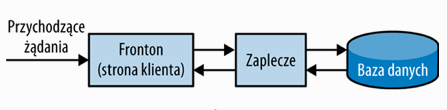
\includegraphics[width=12cm]{Rysunki/Rozdzial1/architektura_trojwarstwowa}
		\caption{Schemat aplikacji trójwarstwowej. Źródło \cite{Folwer:2019}}	
		\label{fig:architekturaTroj}
	\end{figure}

Przykładowe zaplecze oparte~o technologię \textit{LAMP} (ang. \textit{Linux-Apache-MySQL-Perl/PHP/Python)}\cite{Ziade:2018} dla każdej akcji przesłanej przez formularz \textit{HTML} generuje dużą ilość zapytań \textit{SQL} do bazy, a następnie odsyła nowo wygenerowaną stronę uaktualnioną~o żądane informacje\cite{Wilton:2005}. Twórcy takich serwisów zauważyli elementy stałe~w działaniu dla każdego~z nich. Dlatego naturalnym etapem rozwoju takich systemów było opracowanie ogólnodostępnych \textit{frameworków}, czyli zestawu narzędzi~i bibliotek służących do tworzenia podstawy aplikacji. Chcąc przewidzieć jakie problemy napotka programista stosowalni oni ujednolicone architektury, nie tylko jeżeli chodzi~o wzorce programowania, ale też~o cały system, począwszy od kontaktu~z bazą danych, działaniem serwera, sposobu generowania warstwy prezentacji, aż po zarządzaniem wydawania aplikacji~i jej serwowaniem użytkownikom końcowym. Obecnie standardem są dwa główne podejścia, monolityczne~i te oparte~o mikrousługi.

\section{Podejście monolityczne}
Monolit znaczy jednolity blok kamienny\footnote{Źródło: Słownik Języka Polskiego PWN \url{https://sjp.pwn.pl/sjp/monolit;2568347.html}}. Słowo to idealnie oddaje charakter tego typu architektury. Większość takich aplikacji została napisana~w oparciu~o model trójwarstwowy. Z tym, że \textit{fronton}\footnote{Warstwa prezentacji, również nazywana \textit{frontendem}.} (rys. \ref{fig:architekturaTroj}) i zaplecze mają wspólną bazę kodu. Umieszczone są we wspólnym repozytorium~i uruchamiane za pomocą jednego pliku wykonywalnego\cite{Folwer:2019}.

W książce \textit{Rozwijanie mikrousług~w Pythonie}, \textit{Tarek Ziadé} opisuje taką aplikacje na przykładzie agregatora hoteli\cite{Ziade:2018}. Omawiana strona posiada napisaną warstwę prezentacji~w statycznie generowanym \textit{HTML-u}. Użytkownik wchodząc na stronę przesyła zapytania \textit{SQL} do scentralizowanej aplikacji, która następnie prosi zewnętrzne usługi~o listę hoteli. Podczas rejestrowania miejsca~w hotelu kupujący otrzymuje stronę na którą musi się zalogować. Po przesłaniu danych~o płatności serwer komunikuje się~z usługą bankową zewnętrznego dostawcy, następnie informacje~o zakończonej transakcji przekazuje do bazy danych. Aplikacja sprawdza, czy wpis~o zakończeniu płatności jest już zapisana~w usłudze \textit{SQL}, jeśli tak, to na podstawie bazy danych generuje plik \textit{PDF} i przy pomocy \textit{usługi e-mail} przesyła potwierdzenie do użytkownika, sprawdzając jednocześnie informację~o wybranym przez niego hotelu~i również do niego kieruje powiadomienie email~z potwierdzeniem transakcji.

\begin{figure}[h!]
	\centering
		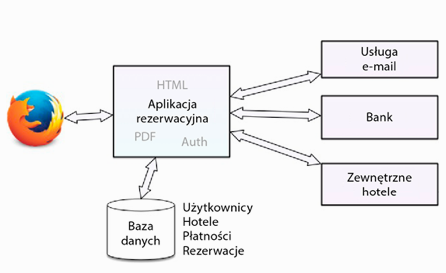
\includegraphics[width=10cm]{Rysunki/Rozdzial1/scentralizowanaArchitektura.png}
		\caption{Schemat scentralizowanej usługi rezerwującej miejsca~w hotelu. Źródło \cite{Ziade:2018}}
		\label{fig:scentralizowanaArchitektura}
\end{figure}

Z opisu jasno wynika, że każda interakcja użytkownika musi mieć swoją odpowiedź idącą~z aplikacji zarządzającej rezerwacjami. Nawet jeśli potrzebuje ona informacji, które bezpośrednio można byłoby otrzymać~z usług zewnętrznych. Tak samo dodatkowe serwisy, odsyłają informację zwrotną jedynie przez aplikacje centralną. Ten przykład dobrze przedstawia idee podejścia monolitycznego, centralnej usługi, która posiada~w sobie wiele przeróżnych funkcji, takich jak autentykacja, generowanie statycznych stron, a nawet plików \textit{PDF}. Wszystkie one są dostępne~w ramach jednej aplikacji, jednolitego bloku kamienia.

\subsection{Założenia aplikacji monolitycznej}
W tego typu aplikacji cała logika zawarta jest~w minimalnie jednym projekcie, który kompilowany jest pojedynczo, a następnie wdrażany jest jako całość. Oddzielanie poszczególnych problemów następuje poprzez grupowanie ich~w osobnych folderach, które~w miarę możliwości powinny izolować dane części aplikacji na \textit{warstwy logiczne}\cite{msbuild}. Założeniem jest wyodrębnienie struktur, które można ponownie używać~w ramach całej aplikacji. Wedle zasady \textit{DRY}\footnote{DRY (ang. \textit{Don't Repeat Yourself}) zasada zalecająca jak najmniejszą powtarzalność tych samych fragmentów kodu~w różnych miejscach aplikacji\cite{hunt:2011}.}. Dodatkowym atutem jest możliwość wymuszania ograniczeń~w sposobie komunikowania się pomiędzy poszczególnymi warstwami, dzięki hermetyzacji kodu\cite{msbuild}. Podstawy podejścia \textit{monolitycznego} są zbudowane na tych samych założeniach, co programowanie obiektowe\cite{Rodger:2019}. Organizacja kodu następuje poprzez hierarchię klas~i \textit{interfejsów}\footnote{W programowaniu obiektowym \textit{interfejsy} odpowiadają za definicję dla grup powiązanych funkcji, które klasa musi zaimplementować\cite{msbuild}.}. Daje to możliwości tworzenia różnych sposobów komunikacji pomiędzy poszczególnymi warstwami~i łatwiejszego wdrażania nowych funkcji. 

\subsection{Architektura aplikacji monolitycznej}
Warstwy logiczne są powszechnie używane przy tworzeniu aplikacji monolitycznych, dlatego powstało wiele technik pozwalających na ich organizację\cite{msbuild}. Najpopularniejszą~z nich jest podzielenie warstw aplikacji na te, które będą odpowiadać za dostęp do danych (\textit{Data Access Layer}), ich zarządzeniem (\textit{Business Logic Layer}) i interakcje~z użytkownikiem (\textit{User Interface}).
\begin{figure}[h!]
	\centering
		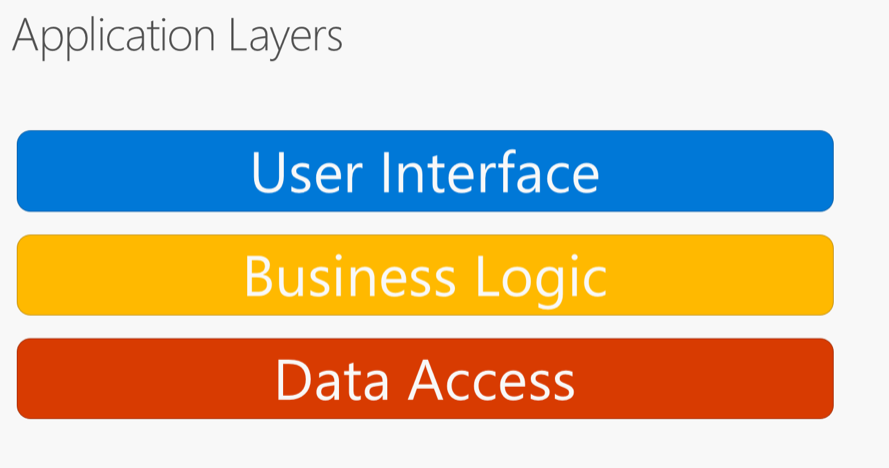
\includegraphics[width=9cm]{Rysunki/Rozdzial1/warstwyAplikacji.png}
		\label{fig:warstwyAplikacji}
	\caption{Struktura warstw aplikacji internetowej. Źródło \cite{msbuild}}
\end{figure}

Dzięki tej architekturze izoluje się możliwości interakcji~z poszczególnymi elementami aplikacji. Użytkownicy wchodzą~w interakcje jedynie~z warstwą \textit{UI}, która następnie współdziedziczy pewne elementy jedynie~z logiką biznesową, gdy zachodzi taka potrzeba, to ona komunikuje się~z warstwą odpowiedzialną za dostęp do bazy danych. Daje to gwarancję, tego, że każda część aplikacji zna dobrze swoje kompetencje~i ogranicza je jedynie do tych, za które jest odpowiedzialna\cite{msbuild}.

Współczesne \textit{frameworki} jeszcze bardziej rozdrabniają poszczególne warstwy, tak, aby udostępnić jedynie programistom \textit{interfejsy} za pomocą, których będą mogli tworzyć swoje aplikacje. \textit{Ruby on Rails} jest oparte~o architekturę \textit{MVC} (ang. \textit{Model-View-Controller}), gdzie modele, są klasami odpowiedzialnymi za interakcję~z dostarczonym przez \textit{framework} mechanizmem kontaktowania się~z bazą danych (\textit{ORMem}\footnote{ORM (ang \textit{Object-Relational Mapping}) system służący za odwzorowanie struktur bazodanowych na struktury programowania obiektowego, tak, aby uprościć tworzenie~i dostęp do bazy danych.}). Kontrolery, których zadaniem jest przyjmowanie danych od użytkownika, modyfikowanie modelu oraz odświeżanie widoków. Natomiast widoki, są odpowiedzialne za wygenerowanie szablonów \textit{HTML} i przesłanie ich do klienta aplikacji (przeglądarki użytkownika)\cite{ruby}.

Jedną~z odnóg architektury \textit{MVC} zastosowano~w \textit{frameworkach} napisany~w języku \textit{Python}, takich jak \textit{Django} i \textit{Flask}. Ich twórcy stworzyli je~w oparciu~o wzorzec \textit{MVT} (ang. \textit{Model-View-Template})\cite{django}, nie różni się on bardzo od pierwowzoru, z tą różnicą, że zamiast klas generujących pliki \textit{HTML}, jego twórcy stworzyli moduł odpowiedzialny za przetwarzanie tego rodzaju plików posiadających specjalne znaczniki (na przykład \textit{Jinja2}\footnote{Więcej~o składni \textit{Jinja2} pod adresem \url{https://jinja.palletsprojects.com/en/2.11.x/}.}). Dostarczają one dodatkowej logiki do interakcji~z danymi przesłanymi przez widok.

\begin{lstlisting}[caption={Przykład szablonu \textit{Django}. Plik \textit{index.html}. Żródło \cite{django}}] 


{{ section.title }}


<h1>{{ section.title }}</h1>


<h2>
  <a href="{{ story.get_absolute_url }}">
    {{ story.headline|upper }}
  </a>
</h2>
<p>{{ story.tease|truncatewords:"100" }}</p>


\end{lstlisting}
Istnieje jeszcze wiele innych podejść do projektowania monolitycznych aplikacji internetowych, te przedstawione tutaj są jednymi~z najpopularniejszych. Jak widać struktury zaprezentowanych \textit{frameworków} internetowych są mocno powiązane~z wcześniej opisanym modelem trójwarstwowym (rys. \ref{fig:architekturaTroj}).

\section{Mikrousługi}
Opozycją do podejścia gdzie, jedna centralna aplikacja, komunikuje się~z zewnętrznymi usługami jest stworzenie kilku mniejszych działających osobno programów. Ich kod można by było podzielić na kilka oddzielnie uruchamianych procesów, które mają odmienne mniejsze zadania do zrealizowania\cite{Ziade:2018}. Wracając do przykładu agregatora hoteli podanego przez \textit{Tarek Ziade}, zamiast jednej usługi odpowiedzialnej za komunikację, generowanie plików, obsługę banku~i e-maili, można byłoby stworzyć wiele mniejszych \textit{mikrousług}.
	
\begin{figure}[h!]
	\centering
		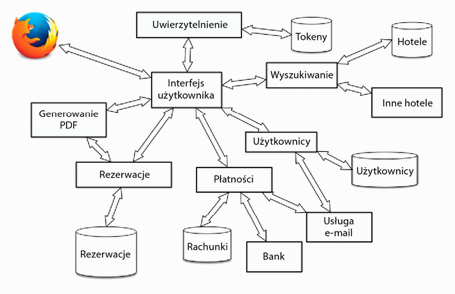
\includegraphics[width=12cm]{Rysunki/Rozdzial1/mikrouslugi}
		\caption{Schemat scentralizowanej aplikacji~z rys. \ref{fig:scentralizowanaArchitektura} oparty~o architekturę mikrousług. Źródło \cite{Ziade:2018}}	
		\label{fig:mikrouslugi}
	\end{figure}
	
Autor książki \textit{Rozwijanie mikrousług~w Pythonie} z powyższego schematu (rys.~\ref{fig:mikrouslugi}), wyodrębnia 7 niezależnych komponentów\cite{Ziade:2018}, takich jak:

\begin{enumerate}
  \item \textbf{Interfejs użytkownika}: frontalną usługę zajmująca się generowaniem \textit{HTMLa} i komunikacją~z innymi procesami.
  \item \textbf{Wyszukiwanie hoteli}: program tworzący listę hoteli na podstawie danych~z zewnętrznych usług.
  \item \textbf{Użytkownicy}: usługa mająca na celu zarządzanie bazą użytkowników~i wysyłaniem do nich wiadomości e-mail.
  \item \textbf{Rezerwacje}: proces odpowiedzialny za zarządzeniu danymi na temat rezerwacji, a także przesyłaniem ich do generatora \textit{PDFów}.
  \item \textbf{Generator PDF}: program generujący na podstawie szablonów~i danych odpowiednio sformatowane pliki \textit{PDF}.
  \item \textbf{Płatności}: moduł komunikujący się~z zewnętrzną usługą banku, również zapisuje informacje~o płatnościach~i wysyła je użytkownikowi~w wiadomości email.
  \item \textbf{Uwierzytelnianie}: usługa generująca \textit{tokeny} stosowane przez inne procesy do uwierzytelniania użytkowników.
 \end{enumerate}
 
 Powyższe mikrousługi mają tą samą funkcjonalność, co aplikacja monolityczna~z rys. \ref{fig:scentralizowanaArchitektura}. Jednak do komunikacji nie wykorzystują elementów programowania obiektowego, a odpowiedni do tego protokół. W tym kontekście każda usługa stanowi osobną logiczną jednostkę odpowiedzialną za jedno ściśle określone zadanie\cite{Ziade:2018}. Takie niezależne usługi nazywane są również komponentami.
  
\subsection{Założenia mikrousług}
Podejście~z wykorzystaniem mikrousług oparte jest~o niewielkie komponenty, które komunikują się~z sobą~w ten sam jednolity sposób bez żadnych przeszkód\cite{Rodger:2019}. \textbf{Niezależnie od warstwy transportowej}, to znaczy, że dane dwie usługi nie muszą nawet wiedzieć~o swoim istnieniu, aby jedna zastąpiła drugą~w przenoszeniu informacji\cite{Rodger:2019}. Wystarczy, że otrzymują~i zwracają odpowiednie komunikaty. Dlatego ważne jest, aby wewnątrz nich znajdowały się informacje~o tym jakie wartości powinny być~w wiadomości zwrotnej, ta cecha to \textbf{dopasowanie do wzorca}. Daje ona możliwość dynamicznego definiowania~z jakiej pomocy innej mikrousługi może skorzystać ta, która obecnie przetwarza informację. Najczęściej~w tym celu stosuje się protokół \textit{HTTP}\cite{http} oparty~o architekturę \textit{REST} (ang. \textit{Representational state transfer}), mającą za zadanie zunifikować odbierane~i wysyłane żądania~w zależności od ich treści\cite{Rodger:2019}. W niezależnych od języka programowania formatach takich jak \textit{JSON}, \textit{XML}, czy \textit{YAML}\cite{Ziade:2018}.

Osiągnięcie pełnej uniwersalności komunikatów nie jest możliwe. Wspomniane wcześniej wzorce muszą być zdefiniowane przez programistów~w ramach architektury \textit{REST}. Każda usługa powinna udostępniać \textit{API} (ang. \textit{Application Programming Interface}), czyli interfejsy, które pomogą innym programistom dostosować się do wzorca komunikatów dla danej usługi\cite{Ziade:2018, Rodger:2019}. To na zespole zajmującym się określony mikroserwisem spoczywa odpowiedzialność za dobrze udokumentowanie \textit{API}, wówczas nie musi się on przejmować wyborem języka programowania, \textit{frameworków}, czy bazy danych\cite{Ziade:2018}.

\begin{figure}[h!]
	\centering
		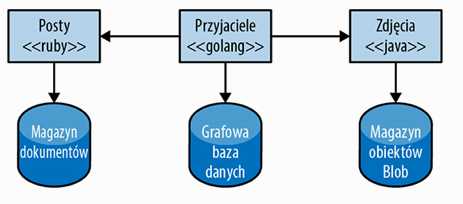
\includegraphics[width=10cm]{Rysunki/Rozdzial1/rozneTechnologie.png}
		\caption{Schemat prezentujący zastosowanie różnych technologii do budowania aplikacji opartych~o mikroserwisy. Źródło \cite{Newman:2016}}	
		\label{fig:rozneTechnologie}
	\end{figure}
	

Z zasady każda usługa powinna być niewielka, ponieważ ma ona ściśle określone cele, a~w razie, gdy będą potrzebne nowe funkcje dla całego systemu, to będzie je można bez przeszkód wprowadzić dodając niezależną jednostkę. Ta charakterystyczna dla mikrousług cecha, to \textbf{addytywność}. Pomaga to~w zapewnieniu dużego~i bardzo skomplikowanego systemu (jako zbioru wszystkich mikrousług) bez większego długu technicznego\cite{Rodger:2019}. W razie potrzeby dowolna jego część jest wymieniana~i zastępowana, bez żadnego ryzyka niestabilnego działania całości aplikacji. Co~w praktyce powinno przekładać się na dużą skalowalność projektu~i jego łatwe wdrożenie\cite{Ziade:2018}.

\subsection{Architektura mikrousług}
Nie ma jednego wzorca pozwalającego określić budowę całego systemu opartego na mikrousługach. W przeciwieństwie do aplikacji monolitycznych, małe niezależne serwisy nie wymagają dogłębnego projektowania hierarchii klas, czy zależności pomiędzy poszczególnymi modułami. W tym wypadku najważniejsze jest spojrzenie na cały system od strony komunikatów, a nie~z perspektywy poszczególnych komponentów. Łatwiej wówczas analizować sposoby interakcji pomiędzy nimi, znajdować odpowiednie wzorce~i dobrze dostosować ich architekturę\cite{Rodger:2019}. Taki pogląd na sytuacje uświadamia, że~w przypadku mikrousług najważniejsze jest dobre zaprojektowanie warstwy transportowej. Wiedza, że poszczególna usługa, to tak naprawdę osobny mini serwer \textit{HTTP} pozwala zwrócić uwagę na ważną cechę~i zarazem niebezpieczeństwo takich jednostek, czyli potrzebę znajomości lokalizacji innej zależnej mikrousługi. W tym celu powinien zostać zaprojektowany proces pozwalający na odnajdowanie innych aplikacji. Rodzi to szereg problemów, ponieważ utrzymywanie takiej usługi nie jest proste, a napisanie dobrej implementacji jest zdaniem dość trudnym\cite{Rodger:2019}. Kolejną sprawą jest to, że przy takim układzie, mikrousługi muszą przechowywać szczegółową wiedzę~o konkretnych serwisach, a to prowadzi do ścisłych zależności. Właśnie tutaj widać fundamentalną różnicę między architekturą mikrousług, a monolitu. Żeby jednolita centralna aplikacja~w którymś~z modułów skorzystała~z metody danej klasy ważne jest, aby posiadała do niej referencję. Z mikrousługami jest podobnie, z tą różnicą, że wszystko odbywa się przez sieć. Dana usługa korzysta~z informacji~o lokalizacji innego serwisu, a także odpowiedniego adresu \textit{URL}, aby skorzystać~z możliwości kolejnej. Odpowiednie zaprojektowanie tej komunikacji ogranicza potrzebę dostarczania dodatkowych usług~i kodu, którego zadaniem byłoby współpracowanie~z mechanizmem wykrywania poszczególnych modułów\cite{Rodger:2019}.
\newpage
W najprostszej konfiguracji mikrousługi komunikują się~z sobą bezpośrednio, ale warto rozszerzyć tą architekturę~o moduły równoważenia obciążenia protokołu \textit{HTTP}, tak zwane \textit{load balancery}. Pozwala to na obsługiwanie ruchu dla różnych instancji mikrousług, a także zapewni proste skalowanie tych usług\cite{Rodger:2019}. Niestety, zwiększy to również złożoność wdrażania takiego systemu.

 \begin{figure}[h!]
	\centering
		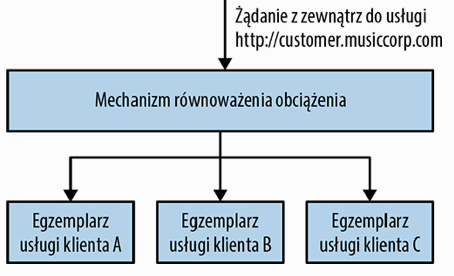
\includegraphics[width=10cm]{Rysunki/Rozdzial1/rownowazenieObciazenia.png}
		\caption{Schemat prezentujący zastosowanie mechanizmu do skalowania liczby instancji usługi klienta. Źródło \cite{Newman:2016}}	
		\label{fig:rownowaznieObciazenia}
	\end{figure}
	
Za jednym \textit{load balancerem} mogą stać różne usługi, ogranicza to czas ich wdrożenia, koszty~i zbędne konfiguracje, ale również może się okazać wąskim gardłem~w działaniu systemu. To~w jaki sposób zostanie wykorzystane narzędzie równoważenia obciążenia zależy od architekta aplikacji~i ma duże znaczenie~w jej działaniu. Ważne jest znalezienie optymalnej konfiguracji~i pokrycie odpowiednich serwisów.
	